  

%%%%%%%%%%%%%%Empieza la presentacion%%%%%%%%%%%%%%%%%%%%%%%%%%%%%%%%%%%%

%\begin{frame}
%\frametitle{Esquema}
 %   \tableofcontents
%\end{frame}

\section{Propiedades de la DFT}


\begin{frame}
\frametitle{Desplazamiento circular I}

\footnotesize

\begin{columns}[T]
\hspace{-0.5cm}\begin{column}{7cm}
\begin{itemize}
\item Señal discreta $x(n)$ $\rightarrow$ Expansión periódica (periodo N) es $x_p(n)\!=\!\sum_{l=-\infty}^{\infty}\!\!x(n\!-\!lN)$
\visible<2->{\item Si la secuencia tiene longitud finita $L<=N$:}
\begin{itemize}
\footnotesize
\visible<3->{\item Su extensión periódica consiste en repetir la señal periódicamente cada N instantes.}
\visible<4->{\item El desplazamiento $x_p(n)$ en el dominio temporal de k unidades  $x_p(n-k)$}\visible<5->{ induce un desplazamiento circular la señal original. }

\item \visible<6->{La señal circular desplazada se representa como $x((n-k)_N)$}.

\scriptsize{


 \visible<7->{
\vspace{0.2cm}

\hspace{-0.4cm}\color{olivegreen}{Ejemplo: $y(n)=x((n-k)_N)$ con  $N=5, k=2$}}

\vspace{0.1cm}

 \visible<8->{
\color{gray}
$y(0)=x((0-2)_5)=x(-2+5)=x(3)$
$y(1)=x((1-2)_5)=x(-1+5)=x(4)$
$y(2)=x((2-2)_5)=x(0)$
$y(3)=x((3-2)_5)=x(1)$
$y(4)=x((4-2)_5)=x(2)$}}


\end{itemize}
\end{itemize}
\end{column}
\hspace{-0.3cm}\begin{column}{4cm}
\only<2|handout:0>{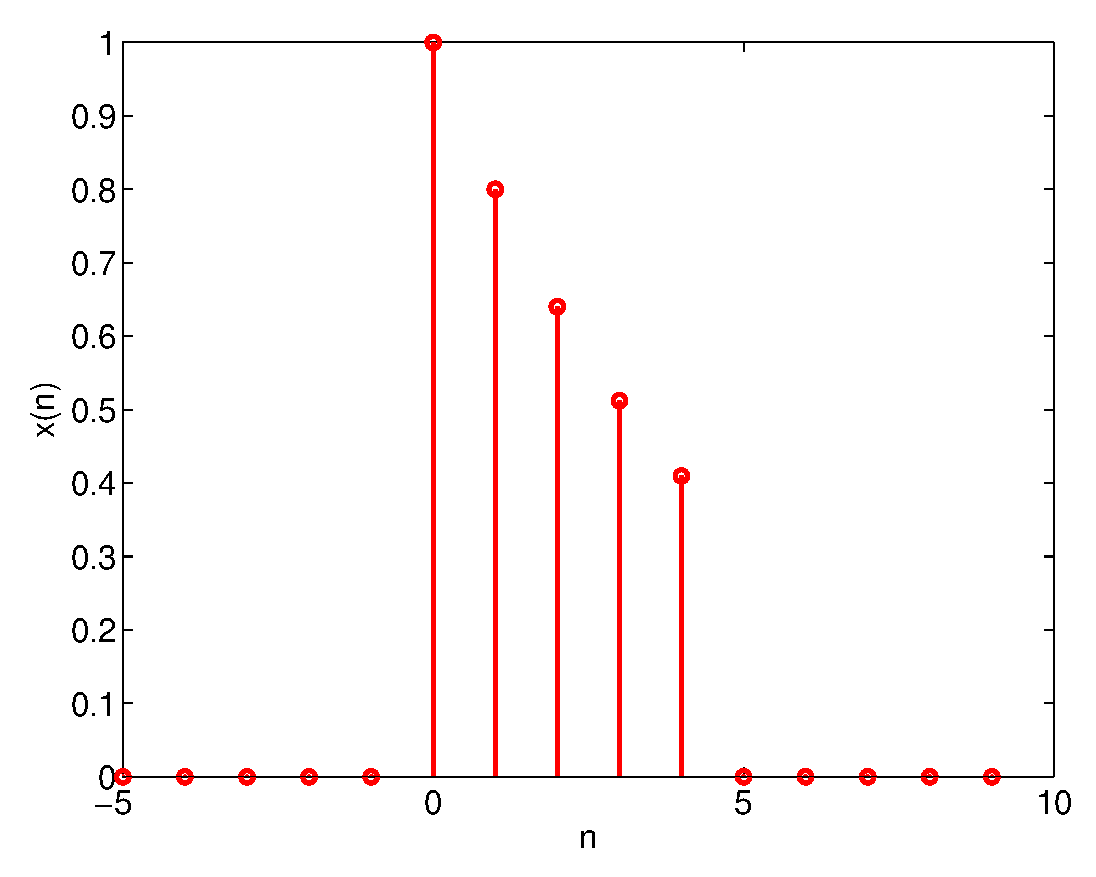
\includegraphics[width=4.5cm]{./Figures/Circular1.eps}}\visible<3->{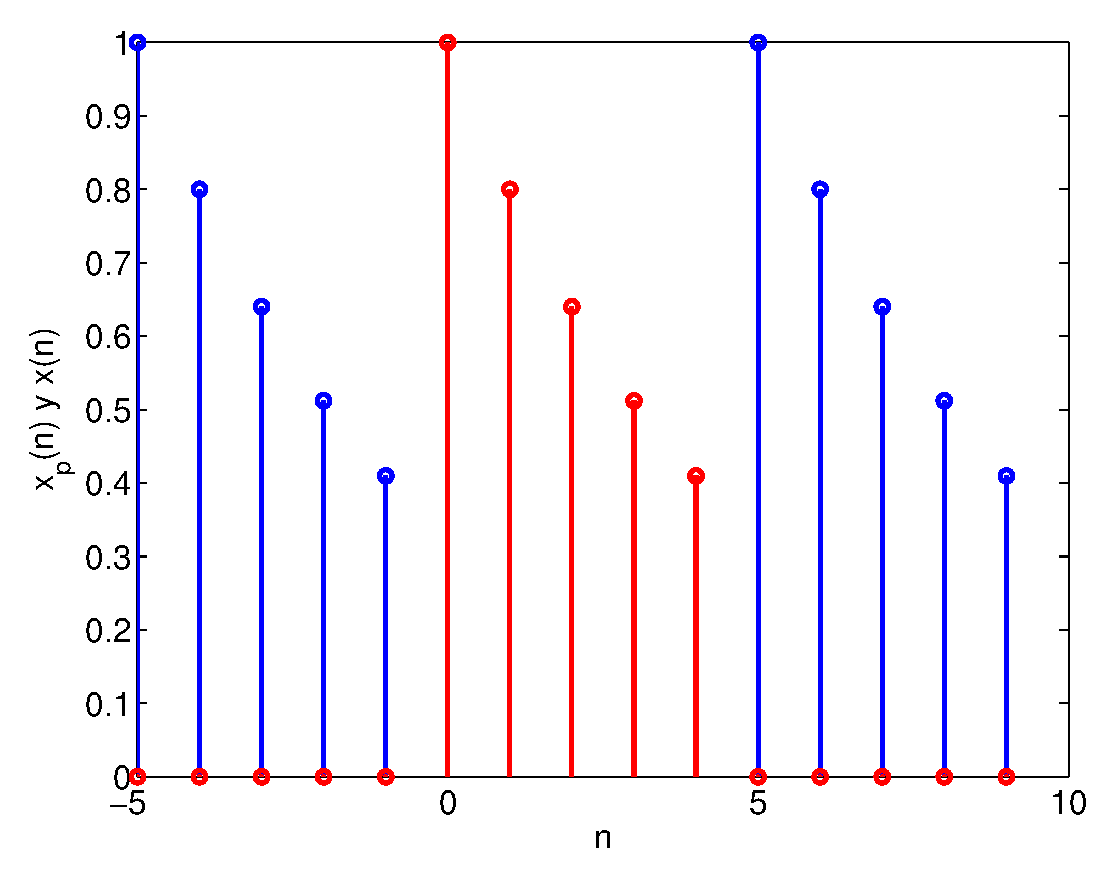
\includegraphics[width=4.5cm]{./Figures/Circular2.eps}}

\only<4|handout:0>{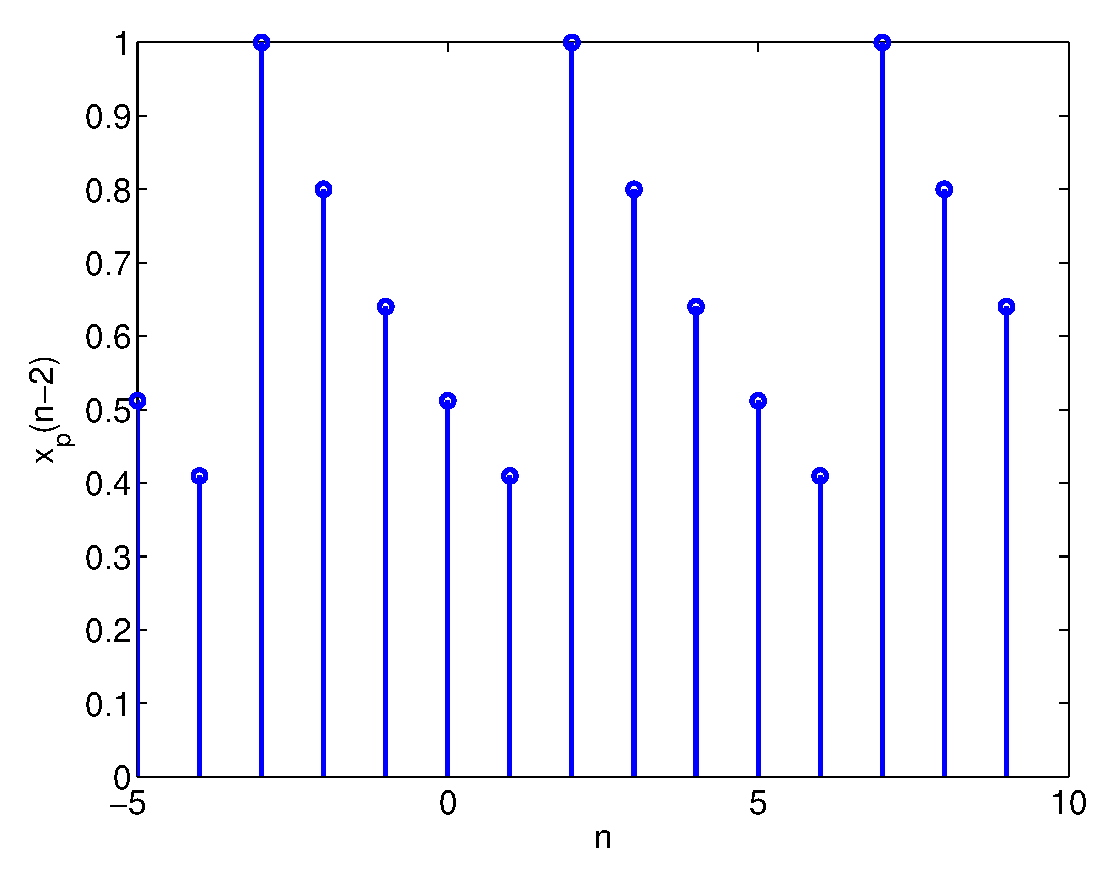
\includegraphics[width=4.5cm]{./Figures/Circular3.eps}}\visible<5->{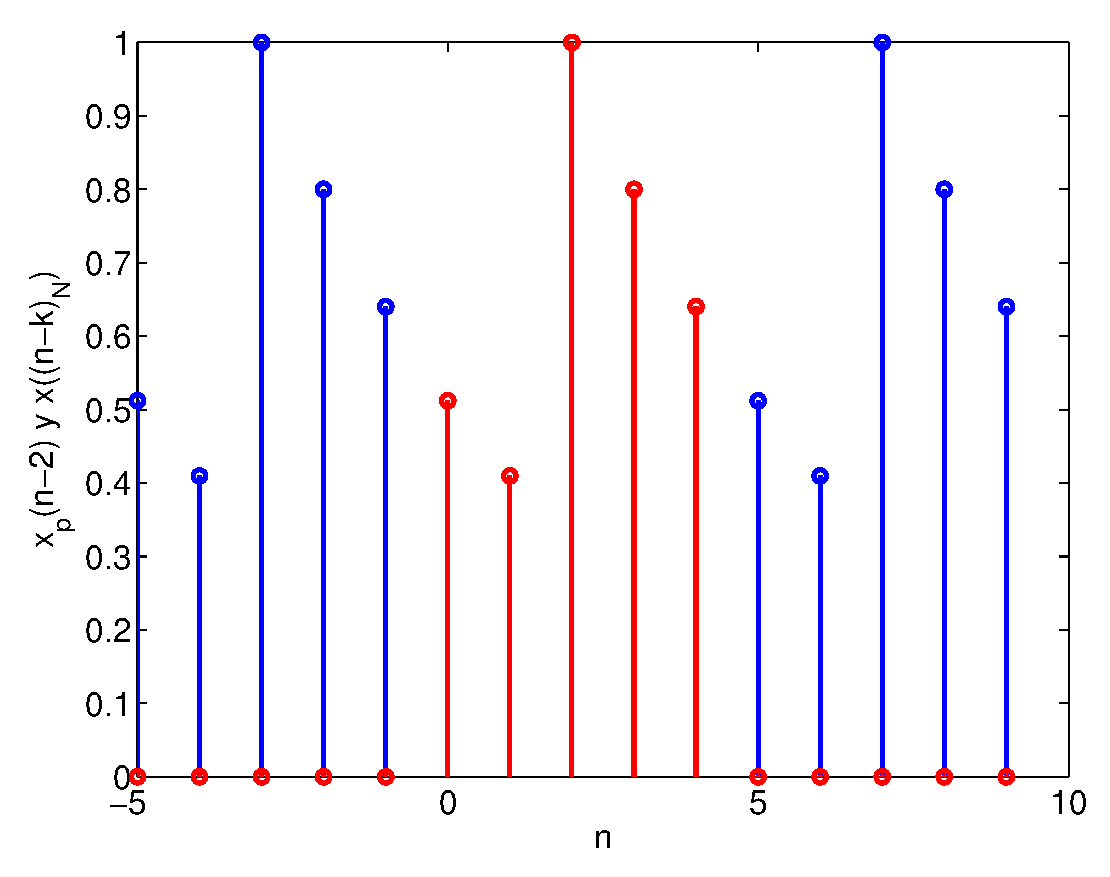
\includegraphics[width=4.5cm]{./Figures/Circular4.eps}}
\end{column}
\end{columns}
\end{frame}

%%%%%%%%%%%%%%%%%%%%%%%%%%%%%%

\begin{frame}
\frametitle{Desplazamiento circular II}

\footnotesize

\begin{itemize}
\item Reflexión temporal: $x((-n)_N)=x(N-n)$
\item Secuencia circularmente par: $x((-n)_N)=x(n)$  
\item Secuencia circularmente impar: $x((-n)_N)=-x(n)$   


\item Propiedades de simetria de la DFT:

\hspace{2cm}\alert{$X(k)=\sum_{n=0}^{N-1} x(n) e^{-j\frac{2\pi}{N}kn}$}

\hspace{2cm}\alert{$x(n)=\frac{1}{N}\sum_{k=0}^{N-1} X(k) e^{j\frac{2\pi}{N}kn}$}


\vspace{0.1cm}

\hspace{2cm}$x(n)=Re[x(n)]+j \: Im[x(n)]=x_p(n)+x_i(n)$

\vspace{0.1cm}

\hspace{5.3cm}$X(k)=X_p(k)+X_i(k)$

\vspace{0.1cm}

\begin{tabular}{|c|c|}

\hline
Secuencia & DFT \\ \hline
$x(n)$ & $X(k)$ \\ \hline
\alert{$x^*(n)$} & \alert{$X^*(N-k)$} \\ \hline
\alert{$x^*(N-n)$} & \alert{$X^*(k)$} \\ \hline
$Re[x(n)]=\frac{x(n)+x^*(n)}{2}$ & $\frac{X(k)+X^*(N-k)}{2}=\frac{X_p(k)+X_i(k)+X_p(N-k)-X_i(N-k)}{2}=X_p(k)$ \\ \hline
$Im[x(n)]=\frac{x(n)-x^*(n)}{2j}$ & $\frac{X(k)-X^*(N-k)}{2j}=\frac{X_p(k)+X_i(k)-X_p(N-k)+X_i(N-k)}{2j}=X_i(k)$ \\ \hline

$x_p(n)=\frac{x(n)+x(N-n)}{2}$ & $\frac{X(k)+X(N-k)}{2}=\frac{X(k)+X^*(k)}{2}=Re[X(k)]$ \\ \hline
$x_i(n)=\frac{x(n)-x(N-n)}{2}$ & $\frac{X(k)-X(N-k)}{2}=\frac{X(k)-X^*(k)}{2}=j \: Im[X(k)]$ \\ \hline

\end{tabular}


\end{itemize}

\end{frame}


%%%%%%%%%%%%%%%%%%%%%%%%%%%%%%%%

\begin{frame}
\frametitle{DFT de señales reales}


\begin{itemize}
\item Se pueden obtener:
\begin{itemize}

\item Utilizando la relación de Euler (tal y como hicimos en el caso de la CTFT y DTFT)
\item Aprovechando la relación entre la DTFT y la DFT, teniendo en cuenta las diferencias de paridad/imparidad habitual y la circular. 
\end{itemize}
\item Propiedades DFT señales reales$^1$:
\begin{itemize}

	\item $x(n) \:\:\: \leftrightarrow \:\:\:X(k)=X^*(N-k)$
	\item La componente real de X(k) es par y la imaginaria es impar.
	\item Si x(n) es par, X(k) es real y par.
	\item Si x(n) es impar, X(k) es imaginaria e impar.
	\item El módulo de X(k) es par y el argumento es impar.
	\item Si x(n) es par, modulo par, argumento es 0 o $\pi$
	\item Si x(n) es impar, modulo par, argumento $\pi/2$ o $3\pi/2$.
\end{itemize}


\end{itemize}

\rule{11cm}{0.4pt}

\footnotesize
$^1$ Con paridad/imparidad circular.

\end{frame}


%%%%%%%%%%%%%%%%%%%%%%%%%%%%%%


\begin{frame}
\frametitle{Propiedades de la DFT}

\small
\hspace{3cm}\alert{\footnotesize $X(k)= \sum_{n=0}^{N-1} x(n) e^{-j\frac{2\pi}{N}kn} $}

\vspace{0.1cm} 
 
\hspace{3cm} \alert{\footnotesize  $x(n)=\frac{1}{N} \sum_{n=0}^{N-1} X(k)  e^{j\frac{2\pi}{N}kn}$}

\vspace{0.2cm}

Propiedades:

\vspace{-0.2cm} 

\begin{itemize}
\footnotesize
\item Linealidad: $\:\:\:\:\:\:\:\:\:\:\:\:\:\:\:\:\:\:\:\:\:\:\:\: \:\:\:\:\:\:\:\:\:\:\:\: \:\:\: \:\:\:\alpha x_1(n)+\beta x_2(n) \:\:\:\: \leftrightarrow  \:\:\:\:\alpha X_1(k)+ \beta X_2(k)$
\item Periodicidad en k: $\:\:\:\:\:\:\:\:\:\:\:\:\:\:\:\:\:\:\:\:\:\:\:\:\:\:\:x(n+N)=x(n)$

\hspace{2cm}$\:\: \:\:\:\:\:\:\:\: \:\:\:\:\:\:\:\: \:\:\:\:\:\:\:\: \:\:\:\:\:\:\:\: X(k)=X(k+N)$

\item Desplazamiento temporal circular: $x((n-l)_N)  \:\:\:\:\:\:\:\: \leftrightarrow   \:\:\:\:\:\:\:\: e^{j\frac{-2\pi}{N}kl}X(k)$
\item Modulación:   $\:\: \:\:\:\:\:\:\:\:\:\:\:\:\:\:\:\:  \:\:\:\:\:\:\:\: \:\:\:\:\:\:\:\:\:\:\:\:\:\:\:\: x(n)e^{j\frac{2\pi}{N}ln}\:\: \:\:\:\:\:\:\:\:  \leftrightarrow \:\:\:\:\:\:\:\: X((k-l)_{N}) $
\item Convolución circular: $\:\:\:\:\:\:\:\:\:\:\:\:\:\:\:\:\:\:\:\:\:\:\:\:\: (x*y)_{N}(n) \:\:\:\:\:\:\:  \leftrightarrow \:\:\:\:\:\:\:\:   X(k)Y(k)$
\item Producto circular: $\:\:\:\:\:\:\:\:\:\:\:\:\:\:\:\:\:\:\:\:\:\:\:\:\:\:\:\:\:\:\: x(n)y(n)   \:\:\: \:\:\:\:\:\:\:\:  \leftrightarrow \:\:\:\:\:\:\:\:  \frac{1}{N}(X*Y)_{N}(k)$

\item $x^*(n) \:\:\:\:\:\:\:\:\:\:\:\:\:\:\:\leftrightarrow \:\:\:\:\:\:\:\:X^*(N-k)$

\item  $x(N-n)  \:\:\:\:\:\:\:\:    \leftrightarrow   \:\:\:\:\:\:\:\:  X(N-k)$

\end{itemize}
\end{frame}
%%%%%%%%%%%%%%%%%%%%%%%%%%%%%%%%%%%%%%%%%%%%%%


\begin{frame}
\frametitle{Convolución circular}

\footnotesize
\begin{itemize}
\item Tenemos dos secuencias finitas de longitud $N$, $x_1(n)$ y $x_2(n)$.
\item Sus DFTs correspondientes son:

\hspace{1cm}$X_1(k)=\sum_{n=0}^{N-1}x_1(n)e^{-j \frac{2\pi}{N}kn}$

\hspace{1cm}$X_2(k)=\sum_{n=0}^{N-1}x_2(n)e^{-j \frac{2\pi}{N}kn}$

\item Definimos producto de ambas señales en el dominio de la transformada $X_3(k)=X_1(k)X_2(k)$.

\item Calculamos la IDFT:
$x_3(m)=\frac{1}{N}\sum_{k=0}^{N-1} X_3(k)e^{j \frac{2\pi}{N}km}=\frac{1}{N}\sum_{k=0}^{N-1} X_1(k)X_2(k)e^{j \frac{2\pi}{N}km}=$
$=\frac{1}{N}\sum_{k=0}^{N-1} \left[\sum_{n=0}^{N-1}x_1(n)e^{-j \frac{2\pi}{N}kn} \right] \left[\sum_{l=0}^{N-1}x_2(l)e^{-j \frac{2\pi}{N}kl} \right]e^{j \frac{2\pi}{N}km}=$
$=\frac{1}{N}\sum_{n=0}^{N-1} x_1(n)  \sum_{l=0}^{N-1}x_2(l) \left[ \sum_{k=0}^{N-1}e^{j \frac{2\pi}{N}k(m-n-l)} \right ]=$
$=\frac{1}{N}\sum_{n=0}^{N-1} x_1(n) N x_2(m-n-pN)=\sum_{n=0}^{N-1} x_1(n) x_2((m-n)|_N)=(x*y)_N(m)$

\item \alert{$(x*y)_N(m)=\sum_{n=0}^{N-1} x_1(n) x_2((m-n)|_N)  \:\:\:\:   \leftrightarrow \:\:\:\: X(k)Y(k)$}

\rule{11cm}{0.4pt}

$\sum_{k=0}^{N-1}e^{j \frac{2\pi}{N}k(m-n-l)} = \left \{\begin{array}{l} N,   \:\:\: m-n-l=pN, p\in \mathcal{Z} \\ 0,  \:\:\: c.c. \end{array}\right .$


\end{itemize}


\end{frame}


\begin{frame}
\frametitle{Relación entre Convoluciones y T. Fourier }

\footnotesize
\begin{itemize}

\item Definiciones de convolución
\begin{itemize}

\footnotesize

\visible<2->{

\item Convolución continua: $(x*y)(t)=\int_{-\infty}^{\infty} x(\tau)y(t-\tau)d\tau$
\item Convolución periódica continua  $(x*y)_T(t)=\int_T x(\tau)y(t-\tau)d\tau$
\item Convolución discreta: $(x*y)(m)=\sum_{n-\infty}^{\infty} x(n)y(m-n)$
\item Convolución circular discreta $(x*y)_N(m)=\sum_{n=0}^{N-1} x(n)y((m-n)|_N)$
}
\end{itemize}

\item Transformadas de Fourier:


\begin{itemize}
\footnotesize
\visible<3->{
\item CTFT:	
\begin{itemize}
	\item Señales genéricas continuas en tiempo y frecuencia.
	\item$\mathcal{F}[(x*y)(t)]=X(jw)Y(jw)$       
	\item $\mathcal{F}[(x(t)y(t))]=\frac{1}{2\pi}(X*Y)(jw)$
\end{itemize}}

\visible<4->{\item DTFT:	
\begin{itemize}
	\item Señal genérica discreta en tiempo y periódica continua en frecuencia.
	\item$\mathcal{F}[(x*y)(n)]=X(e^{jw})Y(e^{jw})$       
	\item $\mathcal{F}[(x(n)y(n))]=\frac{1}{2\pi}(X*Y)_{2\pi}(e^{jw})$
\end{itemize}}

\visible<5->{\item DFT:	
\begin{itemize}
	\item Señal periódica (circular) discreta en tiempo frecuencia.
	\item$\mathcal{F}[(x*y)|_N(n)]=X(k)Y(k)$       
	\item $\mathcal{F}[(x(n)y(n))]=\frac{1}{N}(X*Y)_{N}(k)$
\end{itemize}}

\end{itemize}	


\end{itemize}


\end{frame}

